\begin{problem}{22. Кратчайший путь материальной точки между точками плоскости с полигональными препятствиями}{standard input}{standard output}{2 секунды}{256 мегабайт}

На плоскости заданы две точки: начальное и конечное положение робота. Робот является материальной точкой. Также на плоскости заданы полигональные препятствия. 
Робот должен добраться из начальной точки в конечную по кратчайшему пути, при этом он может касаться препятствий.
Кратчайший путь нужно задать точками, где робот меняет направление своего движения. Гарантируется существования пути и то, что робот изначально находится вне препятствия.
  
\InputFile
В первой строке заданы координаты старта и финиша соответственно.
Во второй строке задано количество препятствий $n$.
Далее следует $n$ блоков, задающих препятствия.
В первой строке каждого блока записано количество вершин $m$ в препятствии. В следующих $m$ строках заданы координаты вершин препятствия.

\OutputFile

В первой строке выходного файла выведите количество поворотов, сделанных роботом -- $k$.
В следующие $k$ строчек выведите координаты точек пути, где робот соверщал поворот. Точки выводятся в порядке обхода. 
Если кратчайших путей несколько, выведите любой из них.
\Examples

\begin{example}%
\exmp{
0.0 0.0 25.0 17.0
2
3
3.0 6.0
7.0 3.0
10.0 8.0
3
21.0 7.0    
20.0 14.0
14.0 12.0
}{
2 
7.0 3.0 
14.0 12.0 
}%
\end{example}

\Note
Пояснение к примеру:
\begin{center}
	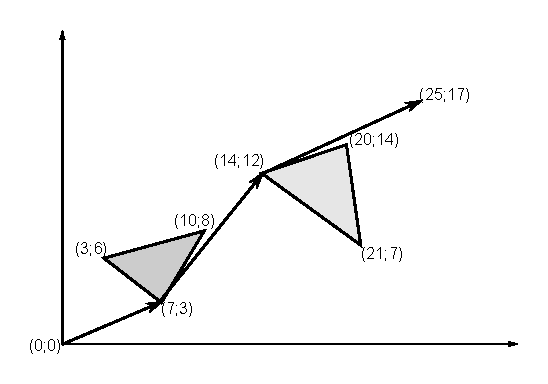
\includegraphics{example.pdf}
\end{center}
\end{problem}